% SkillSpan-layout figures. These commands allow each float to be placed in the
% appropriate manuscript section rather than emitting all five figures together.

\newcommand{\SkillSpanViolinFigure}{%
\begin{figure}[t]
\centering
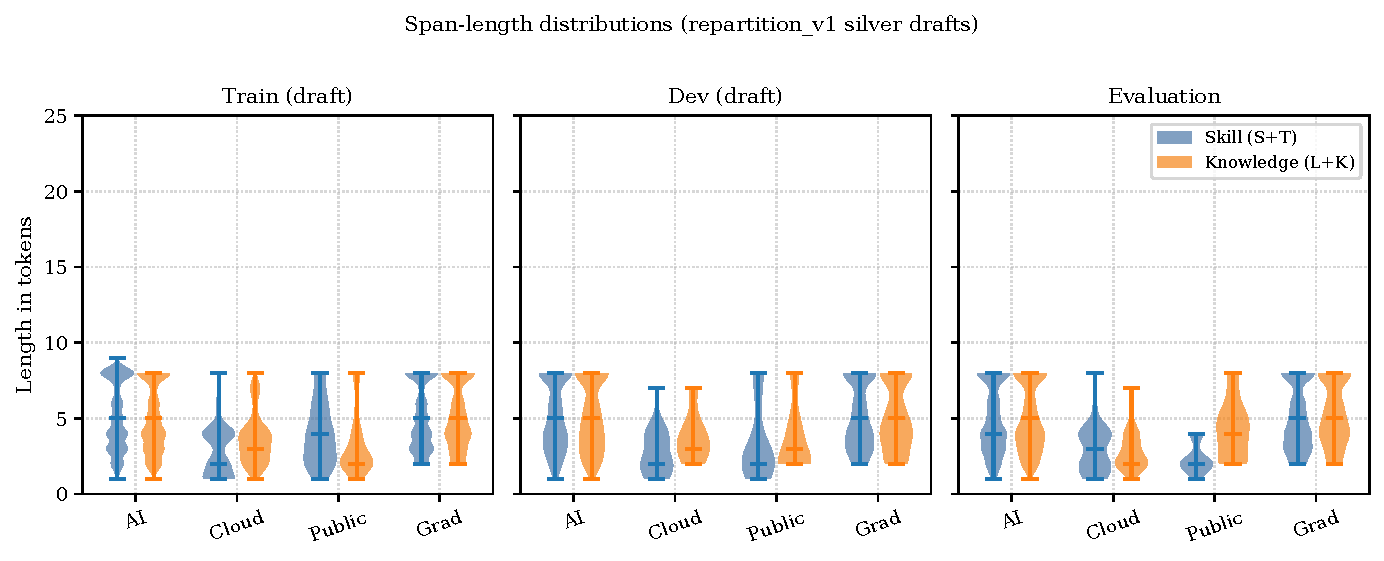
\includegraphics[width=0.96\linewidth]{figures/fig_violin_span_length.pdf}
\caption{Span-length distributions under the official corpus split. Training contains AI and graduate recruitment, development contains AI recruitment, and the 2,601-record evaluation reference contains AI, Cloud, and public-sector recruitment. Skill denotes S+T and Knowledge denotes L+K. Full violins show the complete distributions; white markers denote medians and thick vertical segments denote interquartile ranges. Table~\ref{tab:dataset-stats} instead reports the separate diagnostic repartition.}
\label{fig:violin-spans}
\end{figure}%
}

\newcommand{\StandardizedPerformanceFigure}{%
\begin{figure}[!htbp]
\centering
\includegraphics[width=0.98\linewidth]{figures/fig_standardized_performance.pdf}
\caption{Exact-to-relaxed gain, $\Delta F1=F1_{\mathrm{relaxed}}-F1_{\mathrm{exact}}$, on the archived 2,601-record SOP+jieba reference. The figure derives one boundary-sensitivity diagnostic from the absolute scores in Table~\ref{tab:standardized-benchmark} rather than repeating them. Larger values indicate that overlap-tolerant matching recovers more credit relative to exact typed matching; they are descriptive differences, not uncertainty intervals. These values are not results on the human reference set.}
\label{fig:standardized-performance}
\end{figure}%
}

\newcommand{\StandardizedLabelDomainFigure}{%
\begin{figure*}[!htbp]
\centering
\includegraphics[width=0.90\textwidth]{figures/fig_standardized_label_domain.pdf}
\caption{Archived typed performance by LSKT label and source domain on the 2,601-record SOP+jieba reference, which is distinct from the human reference set. Each cell reports typed exact/typed relaxed micro-F1 and the number of reference spans. Cells with fewer than 10 reference spans are treated as unstable. All eight systems have complete identifier coverage; the comparison is descriptive because encoders use aligned supervision while language models are evaluated zero-shot.}
\label{fig:standardized-label-domain}
\end{figure*}%
}

\newcommand{\StandardizedSpanLengthFigure}{%
% [R1-L01] Flexible placement in the historical appendix.
\begin{figure}[htbp]
\centering
\includegraphics[width=0.96\linewidth]{figures/fig_standardized_span_length.pdf}
\caption{Archived typed exact and relaxed micro-F1 by token-length stratum on the 2,601-record SOP+jieba reference, not the human reference set. Reference and predicted spans are independently binned before matching, so the curves report length-stratified F1 rather than reference-conditioned recall. The unsupported one-token bin is omitted. Separate panels distinguish supervised encoders from zero-shot language models.}
\label{fig:standardized-span-length}
\end{figure}%
}

\newcommand{\SkillSpanSeedWinRateFigure}{%
\begin{figure}[t]
\centering
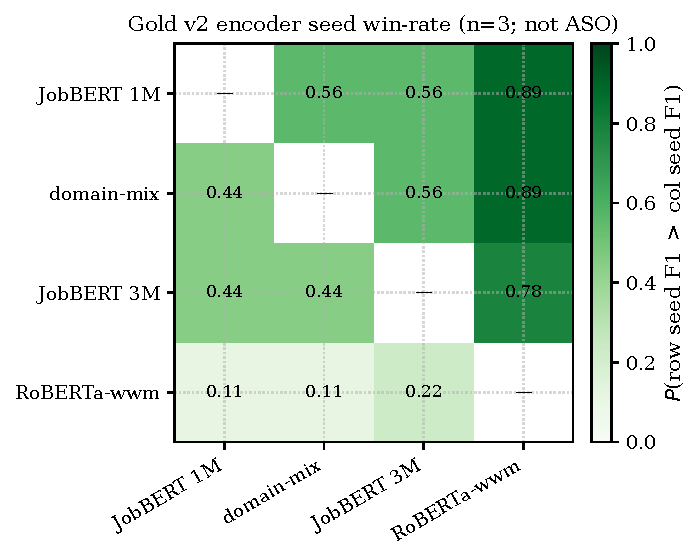
\includegraphics[width=0.72\linewidth]{figures/fig_encoder_seed_winrate.pdf}
\caption{Historical encoder pairwise seed win rate under the earlier annotation convention.
Each cell is $P(F1_{\mathrm{row}}>F1_{\mathrm{column}})$ over $3\times3$ seed pairs. This descriptive analysis uses $n=3$ and is not an Almost Stochastic Order test with Bonferroni correction; it does not reliably separate the 1M, domain-mix, and 3M variants.}
\label{fig:seed-winrate}
\end{figure}%
}

\newcommand{\SkillSpanPredictedLengthFigure}{%
\begin{figure}[t]
\centering
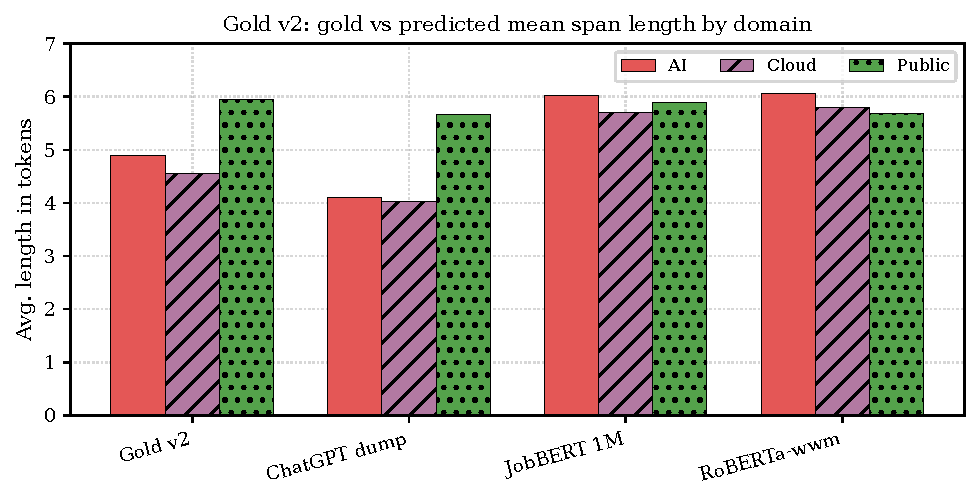
\includegraphics[width=0.92\linewidth]{figures/fig_pred_span_length.pdf}
\caption{Historical mean span length by source domain under the earlier annotation convention.
The encoders predict longer spans (approximately 5.9--6.1 tokens) than the Gold v2 domain means (approximately 4.5--5.9 tokens), whereas the frozen \texttt{gpt-4o} spans more closely match reference length.}
\label{fig:pred-len}
\end{figure}%
}

\newcommand{\SkillSpanFOneByLengthFigure}{%
\begin{figure}[t]
\centering
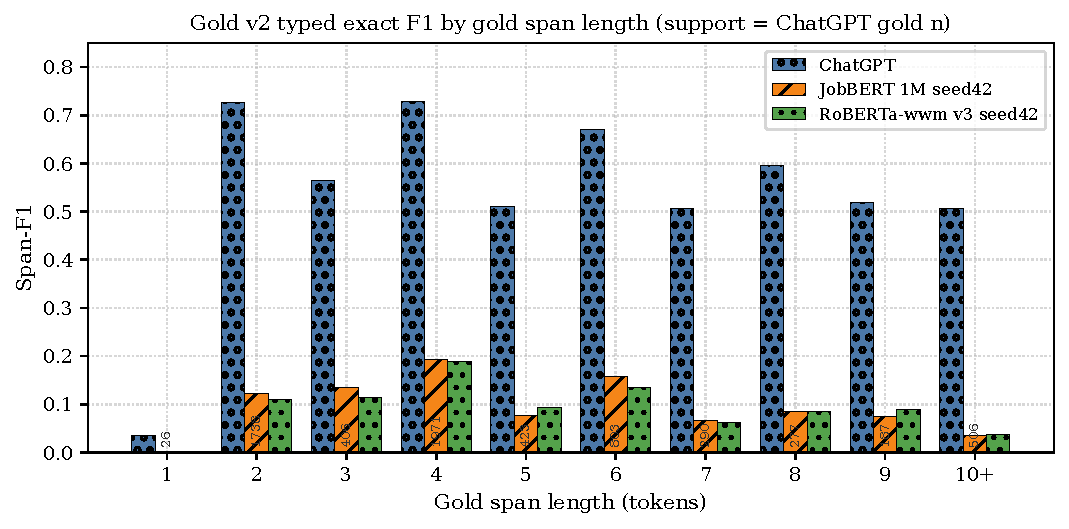
\includegraphics[width=0.98\linewidth,trim=0 0 0 22pt,clip]{figures/fig_f1_by_span_length.pdf}
\caption{Historical typed exact micro-F1 by reference span length under the earlier annotation convention.
Vertical annotations give the number of Gold v2 reference spans in each bucket. The frozen \texttt{gpt-4o} dump is weak on length-one spans but strong at lengths two and four; the two seed-42 encoders remain below 0.20 in every bucket.}
\label{fig:f1-by-len}
\end{figure}%
}
